%
% Copyright 2018 Joel Feldman, Andrew Rechnitzer and Elyse Yeager.
% This work is licensed under a Creative Commons Attribution-NonCommercial-ShareAlike 4.0 International License.
% https://creativecommons.org/licenses/by-nc-sa/4.0/
%
\questionheader{ex:s2.3}
%%%%%%%%%%%%%%%%%%
\subsection*{\Procedural}
%%%%%%%%%%%%%%%%%%


\begin{Mquestion}
Suppose $h(t)$ gives the height at time $t$ of the water at a dam, where the units of $t$ are hours and the units of $h$ are meters.
\begin{enumerate}[(a)]
\item\label{s2.1dam1} What is the physical interpretation of the slope of the secant line through the points $(0,h(0))$ and $(24,h(24))$?
\item\label{s2.1dam2} What is the physical interpretation of the slope of the tangent line to the curve $y=h(t)$ at the point $(0,h(0))$?
\end{enumerate}
\end{Mquestion}
\begin{hint}
Think about units.
\end{hint}
\begin{answer}
\eqref{s2.1dam1} The average rate of change of the height of the water over the single day starting at $t=0$, measured in $\frac{\mathrm{m}}{\mathrm{hr}}$.

\eqref{s2.1dam2} The instantaneous rate of change of the height of the water at the time $t=0$.
\end{answer}
\begin{solution}
\eqref{s2.1dam1} The slope of the secant line is $\dfrac{h(24)-h(0)}{24-0} \quad \dfrac{\mathrm{m}}{\mathrm{hr}}$; this is the change in height over the first day divided by the number of hours in the first day. So, it is the average rate of change of the height over the first day, measured in meters per hour.

\eqref{s2.1dam2} Consider \eqref{s2.1dam1}. The secant line gives the \emph{average} rate of change of the height of the dam; as we let the second point of the secant line get closer and closer to $(0,h(0))$, its slope approximates the instantaneous rate of change of the height of the water. So the slope of the tangent line is the  instantaneous rate of change of the height of the water at the time $t=0$, measured in $\frac{\mathrm{m}}{\mathrm{hr}}$.
\end{solution}

\begin{question}Suppose $p(t)$ is a function that gives the profit generated by selling $t$ widgets. What is the practical interpretation of $p'(t)$?
\end{question}
\begin{answer} Profit per widget
\end{answer}
\begin{solution}
$p'(t) = \displaystyle\lim_{h \rightarrow 0}\frac{p(t+h)-p(t)}{h} \approx \frac{p(t+1)-p(t)}{1} = p(t+1)-p(t)$, or the difference in profit caused by the sale of the $(t+1)^{\mathrm{st}}$ widget. So, $p'(t)$ is the profit from the $(t+1)^{\mathrm{st}}$ widget, so $p'(t)$ is the profit per widget.
\end{solution}

\begin{question} $T(d)$ gives the temperature of water at a particular location $d$ metres below the surface. What is the physical interpretation of $T'(d)$? Would you expect the magnitude of $T'(d)$ to be larger when $d$ is near 0, or when $d$ is very large?
\end{question}
\begin{answer} $T'(d)$ measures how quickly the temperature is changing per unit change of depth, measured in degrees per metre. $|T'(d)|$ will probably be largest when $d$ is near zero, unless there are hot springs or other underwater heat sources.
\end{answer}
\begin{solution} How quickly the temperature is changing per unit change of depth, measured in degrees per metre. In an ordinary body of water, the temperature near the surface ($d=0$) is pretty variable, depending on the sun, but deep down it is more stable (unless there are heat sources). So, one might reasonably expect that $|T'(d)|$ is larger when $d$ is near 0.
\end{solution}

\begin{question}$C(w)$ gives the calories in $w$ grams of a particular dish. What does $C'(w)$ describe?
\end{question}
\begin{answer} Calories per gram.
\end{answer}
\begin{solution} $C'(w)=\displaystyle\lim_{h \rightarrow 0} \dfrac{C(w+h)-C(w)}{h} \approx \dfrac{C(w+1)-C(w)}{1}=C(w+1)-C(w)$, which is the number of calories in $C(w+1)$ grams minus the number of calories in $C(w)$ grams. This is the number of calories per gram.
\end{solution}

\begin{Mquestion}The velocity of a moving object at time $t$ is given by $v(t)$. What is $v'(t)$?
\end{Mquestion}
\begin{answer} The acceleration of the object.
\end{answer}
\begin{solution} The rate of change of velocity is acceleration. (If your velocity is increasing, you're accelerating; if your velocity is decreasing, you have negative acceleration.)
\end{solution}


\begin{Mquestion}
The function $T(j)$ gives the temperature in degrees Celsius of a cup of water after $j$ joules of heat have been added. What is $T'(j)$?
\end{Mquestion}
\begin{answer} Degrees Celsius temperature change per joule of heat added.
(This is closely related to heat capacity and to
         specific heat --- there's a nice explanation of this on Wikipedia.)
\end{answer}
\begin{solution}
The rate of change in this case will be the relationship between the heat added and the temperature change. $\displaystyle\lim_{h \rightarrow 0} \dfrac{T(j+h)-T(j)}{h} \approx \dfrac{T(j+1)-T(j)}{1}=T(j+1)-T(j)$, or the change in temperature after the application of one joule. (This is closely related to heat capacity and to
         specific heat --- there's a nice explanation of this on Wikipedia.)
\end{solution}


\begin{Mquestion}\label{s2.3bacteria}A population of bacteria, left for a fixed amount of time at temperature $T$, grows to $P(T)$ individuals. Interpret $P'(T)$.
\end{Mquestion}
\begin{answer} Number of bacteria added per degree. That is: the number of extra bacteria (possibly negative) that will exist in the population by raising the temperature by one degree.
\end{answer}
\begin{solution} As usual, it is instructive to think about the definition of the derivative:
\[P'(T) = \displaystyle\lim_{h \rightarrow 0}\dfrac{P(T+h)=P(T)}{h} \approx \dfrac{P(T+1)-P(t)}{1} = P(T+1)-P(T).\] This is the difference in population between two hypothetical populations, raised one degree in temperature apart. So, it is the number of extra individuals that exist in the hotter experiment (with the understanding that this number could be negative, as one would expect in conditions that are hotter than the bacteria prefer). So $P'(T)$ is the number of bacteria added to the colony per degree.
\end{solution}

%%%%%%%%%%%%%%%%%%
\subsection*{\Application}
%%%%%%%%%%%%%%%%%%

\begin{question} You hammer a small nail into a wooden wagon wheel. $R(t)$ gives the number of rotations the nail has undergone $t$ seconds after the wagon started to roll. Give an equation for how quickly the nail is rotating, measured in degrees per second.
\end{question}
\begin{hint} There are 360 degrees in one rotation.
\end{hint}
\begin{answer} $360R'(t)$
\end{answer}
\begin{solution}
$R'(t)$ is the rate at which the wheel is rotating measured in rotations per second. To convert to degrees, we multiply by 360: $\boxed{360R'(t)}$.
\end{solution}

\begin{Mquestion}A population of bacteria, left for a fixed amount of time at temperature $T$, grows to $P(T)$ individuals. There is one ideal temperature where the bacteria population grows largest, and the closer the sample is to that temperature, the larger the population is (unless the temperature is so extreme that it causes all the bacteria to die by freezing or boiling). How will $P'(T)$ tell you whether you are colder or hotter than the ideal temperature?
\end{Mquestion}
\begin{hint} $P'(t)$ was discussed in Question~\ref{s2.3bacteria}.
\end{hint}
\begin{answer}  If $P'(t)$ is positive, your sample is below the ideal temperature, and if $P'(t)$ is negative, your sample is above the ideal temperature. If $P'(t) = 0$, you don't know whether the sample is exactly at the ideal temperature, or way above or below it with no living bacteria.
\end{answer}
\begin{solution} If $P'(t)$ is positive, your sample is below the ideal temperature, because
adding heat increases the population. If $P'(t)$ is negative, your sample is above the ideal temperature, because adding heat decreases the population. If $P'(t)=0$, then adding a little bit of heat doesn't change the population, but it's unclear why this is. Perhaps your sample is deeply frozen, and adding heat doesn't change the fact that your population is 0. Perhaps your sample is boiling, and again, changing the heat a little will keep the population constant at ``none." But also, at the ideal temperature, you would expect $P'(t)=0$. This is best seen by noting in the curve below, the tangent line is horizontal at the peak.
\begin{center}
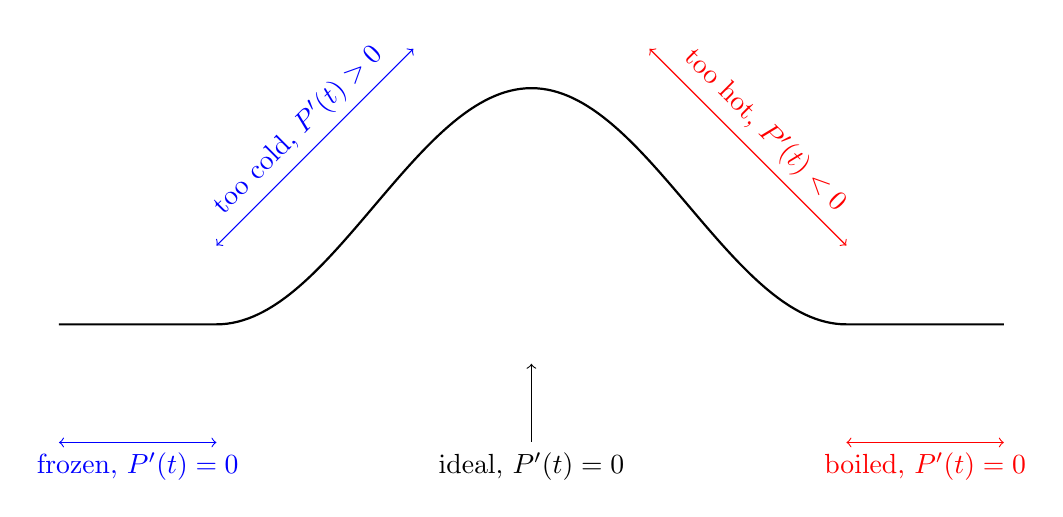
\begin{tikzpicture}
\YEaaxis{1}{12}{1}{3}
\draw[thick] (0,0)--(2,0) cos (4,1.5) sin (6,3) cos (8,1.5) sin (10,0)--(12,0);
\draw[<->, blue] (0,-1.5)--(2,-1.5) node[midway, below]{frozen, $P'(t)=0$};
\draw[<->, red] (10,-1.5)--(12,-1.5) node[midway, below]{boiled, $P'(t)=0$};
\draw[<-] (6,-.5)--(6,-1.5) node[below]{ideal, $P'(t)=0$};
\draw[<->, blue] (2,1)--(4.5,3.5) node[midway, above, rotate=45]{too cold, $P'(t)>0$};
\draw[<->, red] (7.5,3.5)--(10,1) node[midway, above, rotate=-45]{too hot, $P'(t)<0$};
\end{tikzpicture}
\end{center}
\end{solution}
